% --- Inference optimisation: KV caching and serving levers ---
\begin{frame}{Inference Optimisation: Key-Value Caching}
  \begin{columns}[T,onlytextwidth]
    \column{0.48\textwidth}
    \begin{itemize}\footnotesize
      \item[\textcolor{red}{$\blacktriangleright$}] In \textbf{decode}, the model emits \textbf{one token per step}, but that token still depends on the \textbf{key and value} tensors for \textbf{all} earlier positions.
      \item[\textcolor{red}{$\blacktriangleright$}] Those positions include the \textbf{prompt} (K/V from \textbf{prefill}) plus any \textbf{new} K/V computed up to the current step.
      \item[\textcolor{red}{$\blacktriangleright$}] \textbf{KV caching} keeps these tensors in GPU memory so they are \textbf{not recomputed} at every step; each iteration \textbf{appends} the newly computed K/V to the cache for the next step.
      \item[\textcolor{red}{$\blacktriangleright$}] In many stacks there is \textbf{one KV cache per transformer layer}.
    \end{itemize}

    \column{0.5\textwidth}
    \centering
    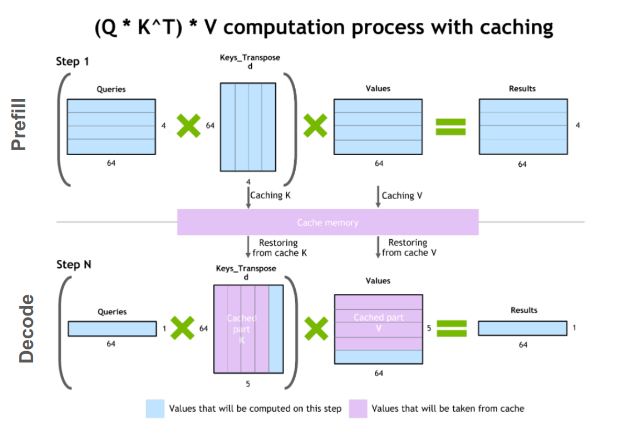
\includegraphics[width=0.8\linewidth,height=0.78\textheight,keepaspectratio]{assets/New-Lecture-Inference_Optimisation/nvidia_blog_kv_caching_figure1.png}\\[-0.2em]
    {\scriptsize Figure: illustration of the key-value caching mechanism. Reference: Verma \& Vaidya, ``Mastering LLM Techniques: Inference Optimization,'' NVIDIA Technical Blog (2023).}
  \end{columns}
\end{frame}

\begin{frame}{KV Cache Memory}
  \begin{columns}[T,onlytextwidth]
    \column{0.52\textwidth}
    \begin{itemize}\footnotesize
      \item[\textcolor{red}{$\blacktriangleright$}] With batching, each request needs its own KV cache, which can become a bottleneck even before model weights do.
      \item[\textcolor{red}{$\blacktriangleright$}] Cost increases in proportion to batch size and sequence length, limiting throughput and ability to handle long inputs. This drives use of techniques like MQA/GQA, paging (PagedAttention), and KV quantization. 
      \end{itemize}
    \column{0.47\textwidth}
    \centering
    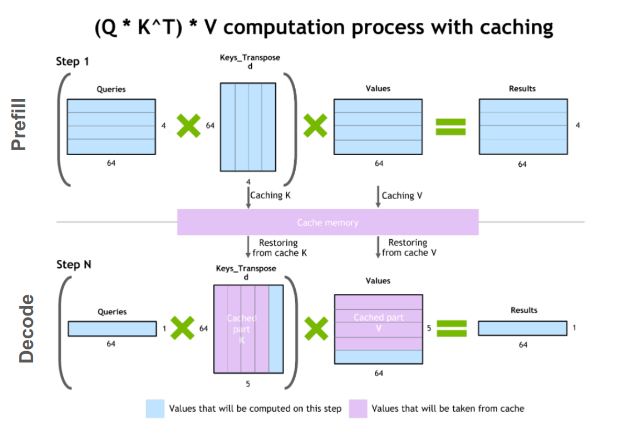
\includegraphics[width=0.8\linewidth,height=0.78\textheight,keepaspectratio]{assets/New-Lecture-Inference_Optimisation/nvidia_blog_kv_caching_figure1.png}\\[-0.2em]
    {\scriptsize Figure: illustration of the key-value caching mechanism. Reference: Verma \& Vaidya, ``Mastering LLM Techniques: Inference Optimization,'' NVIDIA Technical Blog (2023).}
  \end{columns}
\end{frame}

\begin{frame}{Other Inference Levers}
  \begin{itemize}
    \item[\textcolor{red}{$\blacktriangleright$}] \textbf{Kernel fusion \& IO-aware attention} (e.g.\ FlashAttention-style): reduce HBM traffic.
    \item[\textcolor{red}{$\blacktriangleright$}] \textbf{Batching / continuous batching:} pack requests to improve GPU utilisation.
    \item[\textcolor{red}{$\blacktriangleright$}] \textbf{Weight sharing / low-rank adapters (LoRA):} smaller footprints where applicable.
    \item[\textcolor{red}{$\blacktriangleright$}] \textbf{Approximate attention} (long contexts): trade accuracy for sub-quadratic cost.
  \end{itemize}
\end{frame}

% \begin{frame}{Speculative Decoding}
%   \begin{columns}[T,onlytextwidth]
%     \column{0.44\textwidth}
%     \begin{itemize}\itemsep0.3em
%       \item[\textcolor{red}{$\blacktriangleright$}] Use a \textbf{small draft model} to propose several tokens; the \textbf{large target model} verifies in parallel.
%       \item[\textcolor{red}{$\blacktriangleright$}] Accepts a prefix of draft tokens when probabilities align; \textbf{no change} in the target distribution when implemented correctly.
%       \item[\textcolor{red}{$\blacktriangleright$}] Speedups when draft acceptance is high and verification is cheaper than serial decoding.
%     \end{itemize}
%     \column{0.54\textwidth}
%     \centering
%     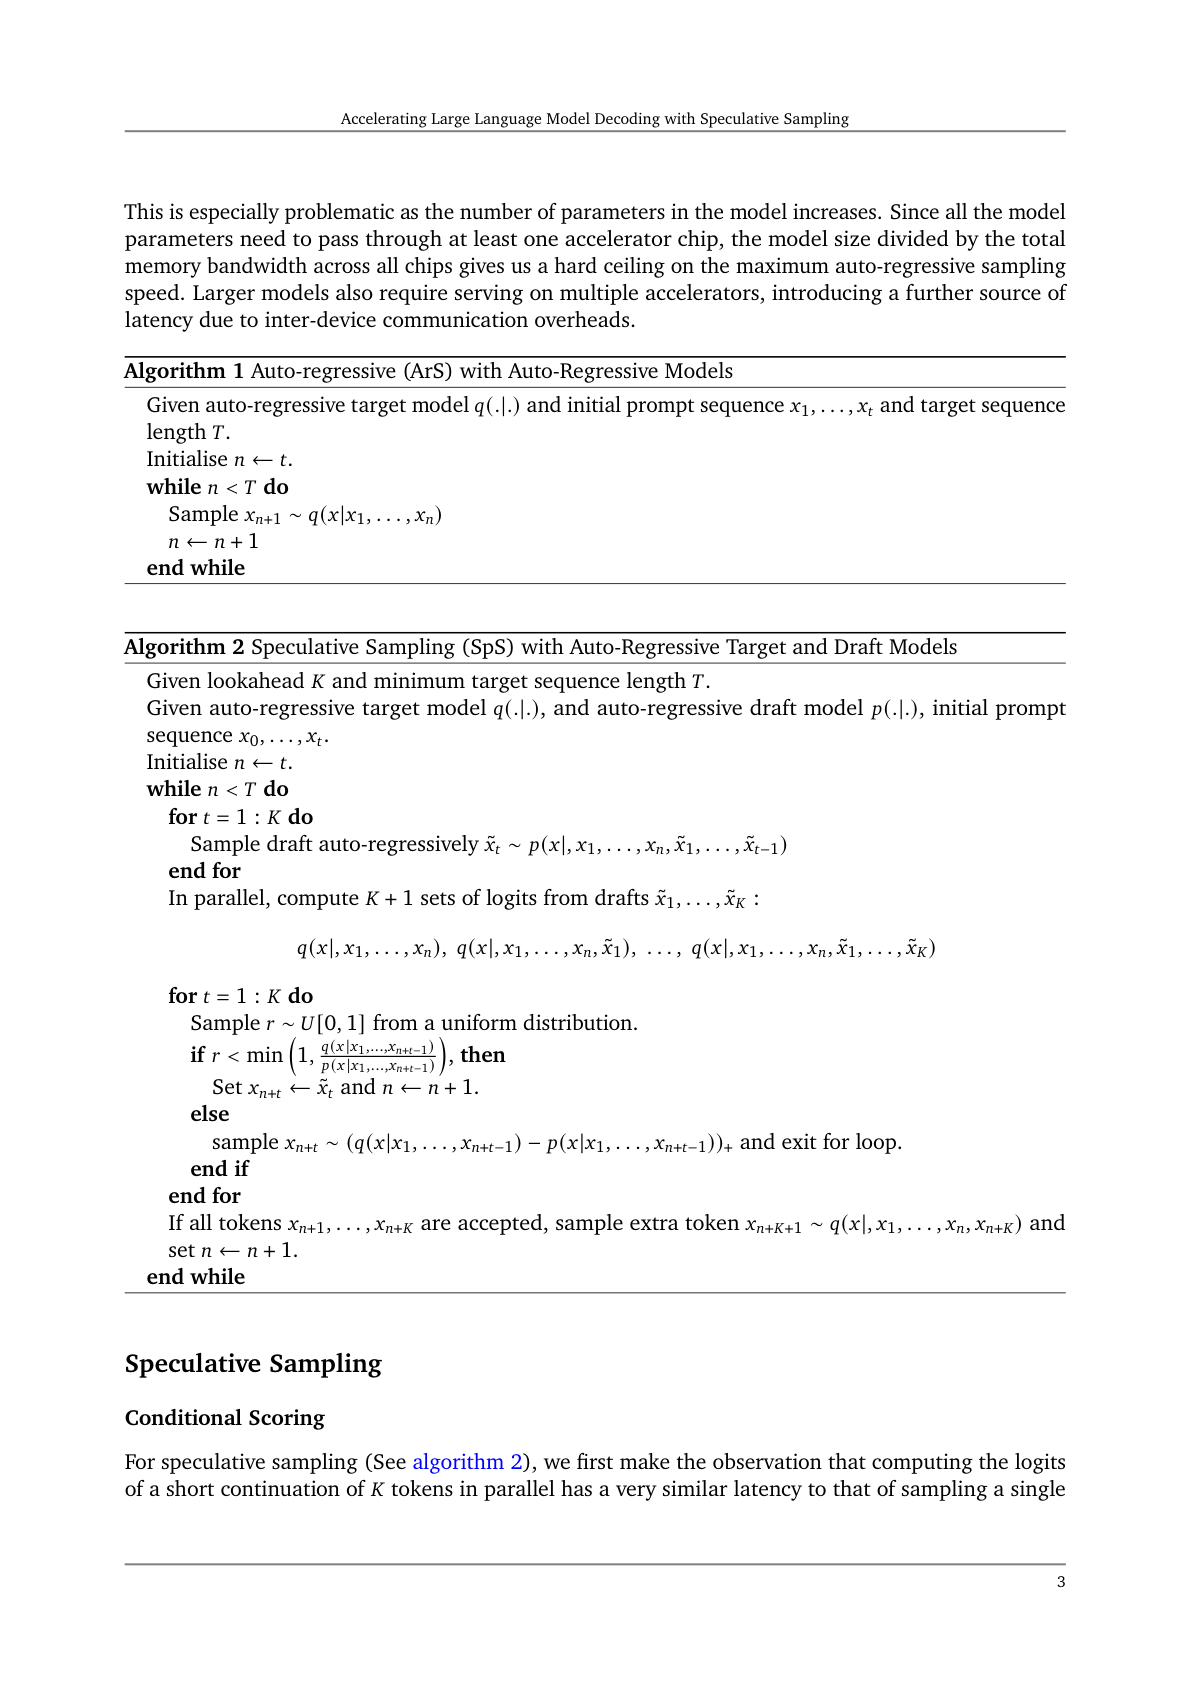
\includegraphics[width=\linewidth,height=0.8\textheight,keepaspectratio]{assets/New-Lecture-Inference_Optimisation/speculative_decoding_p3.png}\\[-0.2em]
%     {\scriptsize Speculative sampling (Leviathan et al.; matching figure from PDF).}
%   \end{columns}
% \end{frame}
